\title{Projections}
\subtitle{\SubTitleName}
\institute[]{\Course}
\author{\Instructor}
\maketitle   
  

 
\begin{frame}\frametitle{Topics and Objectives}
\Emph{Topics} \\
%\TopicStatement
\begin{itemize}

    \item orthogonal projections
    
\end{itemize}

\vspace{0.5cm}

\Emph{Learning Objectives}\\

\LearningObjectiveStatement

\begin{itemize}
    \item compute orthogonal projections and distances between points and lines
    
    % \item express a vector as a linear combination of orthogonal vectors
    % \item characterize bases for subspaces of $\mathbb R^n$, and

\end{itemize}

\end{frame}






\begin{frame}{Motivating Questions}

    Suppose $\vec y$ and $\vec u$ are non-zero vectors in $\mathbb R^n$, and $W$ to be the span of $\vec u$. 
    
    \begin{itemize}
        \item<2-> Let the closest vector in $W$ to $\vec y$ be $\widehat y$. How can we identify $\widehat y$? 
        \item<3-> We would like to write $\vec y = \widehat y + \vec z$, where $\vec z \in W\Perp$. How do we identify vectors $\widehat y$ and $\vec z$? 
    \end{itemize}
    
    \onslide<4->{These two questions are closely related. A sketch of what we are looking for: }
    \begin{center}
        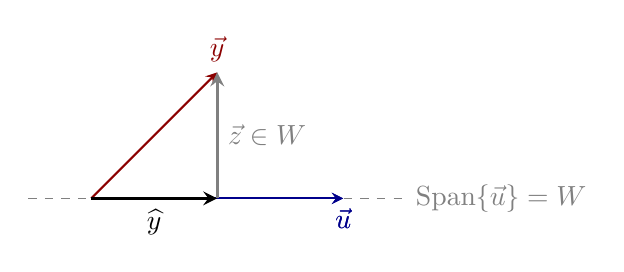
\begin{tikzpicture}[scale=.8] 
            \onslide<5->{
            \draw[->,DarkRed, thick,-stealth] (0,0) -- (2,2) node[above] {$ \vec y$}; 
            \draw[->,DarkBlue, thick,-stealth] (0,0) -- (4,0) node[below] {$ \vec u$}; 
            }
            \onslide<6->{
            \draw[-,gray, dashed] (-1,0) -- (5,0) node[below, right] {Span$\{\vec u\} = W$}; 
            \draw[->,DarkBlue, thick,-stealth] (0,0) -- (4,0) node[below] {$ \vec u$}; 
            }            
            \onslide<7->{
            \draw[->,black, very thick,-stealth] (0,0) -- (2,0) node[midway,below] {$\widehat y$}; 
            }
            \onslide<8->{
            \draw[->,gray, very thick,-stealth] (2,0) -- (2,2) node[midway,right] {$\vec z \in W\Perp$}; 
            }
        \end{tikzpicture}
    \end{center}

\end{frame}

\begin{frame}{For What $\widehat y$ is $\vec z \in W\Perp$?}

   We wish to write $\vec y = \widehat y + \vec z$, where $\vec u \in W$, and $\vec z \in W\Perp$. \onslide<2->{ If $\vec z$ is in $W\Perp$, then }
   \begin{align*}
       \onslide<3->{0 & = \vec z \cdot \vec u}
   \end{align*}
    \onslide<4->{Given some real number $k$, $\vec z = \vec y - k \vec u$, so}
   \begin{align*}
       \onslide<5->{0 & = (\vec y - k \vec u) \cdot \vec u \\}
       \onslide<6->{ & = \vec y\cdot \vec u - k \vec u\cdot \vec u \\}
       \onslide<7->{ k & = \frac{\vec y\cdot \vec u}{ \vec u\cdot \vec u}, \quad \vec u \ne \vec 0}
   \end{align*}    
   \onslide<8->{Thus, the closest vector in the span of $\vec u$ is $$\widehat y = \frac{\vec y\cdot \vec u}{ \vec u\cdot \vec u} \vec u$$}
\end{frame}


\begin{frame}{An Orthogonal Projection}

    \begin{center}\begin{tikzpicture} \node [mybox](box){\begin{minipage}{0.85\textwidth}\vspace{4pt}
    Let $ \vec u$ be a non-zero vector in $\mathbb R^n$, and let $ \vec y$ be any vector in $\mathbb R^n$.  The \Emph{orthogonal projection of $ \vec y$ onto $ \vec u$} is the vector in the span of $ \vec u$ that is closest to $ \vec y$. 
    \begin{equation*}
        \textup{proj} _{\vec u} \, \vec y = \frac {\vec y \cdot \vec u} {\vec u \cdot \vec u} \vec u 
    \end{equation*}
    Moreover, $\vec y = \widehat y + \vec z$, where $\vec z \in W\Perp$. 
    \end{minipage}}; \node[fancytitle, right=10pt] at (box.north west) {Theorem};\end{tikzpicture}\end{center}


\end{frame}






\begin{frame}{Geometric Interpretation}

    The vector $ \vec z =  \vec y - \textup{proj} _{\vec u} \vec y$ is orthogonal to $ \vec u$, so that 
    \pause
            \begin{gather*}
                \vec y =  \textup{proj} _{\vec u} \vec y  + \vec z \\
                \lVert \vec y \rVert ^2 
                = \lVert \textup{proj} _{\vec u} \vec y\rVert ^2 
                + \lVert \vec z \rVert ^2  
            \end{gather*}
            
    \pause
        Schematic:
        \pause 
            \vspace{-12pt}
            \begin{center}
            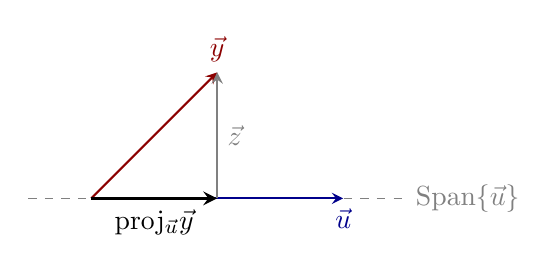
\begin{tikzpicture}[scale=.8] 
                \draw[-,gray, dashed] (-1,0) -- (5,0) node[below, right] {Span$\{\vec u\}$}; 
                \draw[->,DarkBlue, thick,-stealth] (0,0) -- (4,0) node[below] {$ \vec u$}; 
                \draw[->,DarkRed, thick,-stealth] (0,0) -- (2,2) node[above] {$ \vec y$}; 
                \draw[->,black, very thick,-stealth] (0,0) -- (2,0) node[midway,below] {proj$_{\vec u} \vec y$}; 
                \draw[->,thick,gray,-stealth] (2,0) -- (2,2) node[midway,right] {$\vec z$};
            \end{tikzpicture}
            \end{center} 
\end{frame}






\begin{frame}{Example: Projection onto Orthogonal Compliment}  

    True or false: if $\vec u$ is in one-dimensional subspace $S$, and $S\Perp$ is also a one-dimensional subspace, then the projection of $\vec u$ onto $S^{\perp}$ is $\vec{0}$.
\end{frame}







\begin{frame}{Example: Computing Projections and Distances}  

    Suppose $ L$ is the line spanned by $ \vec u$. 
    
    $$\vec u = \spalignmat{1;1;1}, \qquad \vec y = \spalignmat{3;4;2}  $$
    \begin{enumerate}
        \item Calculate the projection of $ \vec y$ onto line $ L$.  
        \item What is the distance between $ \vec y $ and line $L$? 
    \end{enumerate}
    %% ENUMERATE
    \vspace{2in} 
\end{frame}





\frame{\frametitle{Summary}

    \SummaryLine \vspace{4pt}
    \begin{itemize}\setlength{\itemsep}{8pt}

    \item computing orthogonal projections 
    \item computing distances between points and lines
    
    \end{itemize}
    
    \vspace{8pt}
    
}



